\documentclass[10pt,utf8,presentation,notheorems,xcolor=dvipsnames,compress]{beamer}
\usepackage{doclad}

\newcommand{\ov}{\overline}
\newcommand{\fr}{\cfrac}
\newcommand{\ti}{\times}
\newcommand{\ttt}{\theta}
\newcommand{\wt}{\widetilde}

\newcommand{\lwo}{\widetilde{\overline{\lambda}}}%лямбда волна черта
\newcommand{\lw}{\overline{\lambda}}%лямбда черта
\newcommand{\lo}{\lambda_{0}}%лямбда о
\newcommand{\lnw}{\overline{\lambda}_{\nu}} %лямбда ню черта

\newcommand{\mwo}{\widetilde{\overline{\mu}}} %мю волна черта
\newcommand{\mw}{\overline{\mu}} %мю черта
\newcommand{\mo}{\mu_{\o}} %мю  о
\newcommand{\mnw}{\overline{\mu}_{\nu}} %мю ню черта

\newcommand{\ow}{\overline{\omega}}%омега черта
\newcommand{\rw}{\overline{r}}%r черта
\newcommand{\rrw}{\overline{r'}}%r' черта
\newcommand{\ew}{\overline{e}}%e черта
\newcommand{\vw}{\overline{v}}%v черта
\newcommand{\pw}{\overline{\rho}}%rho черта
\newcommand{\ppw}{\overline{\rho'}}%rho' черта
\newcommand{\Dt}{\Delta t}%delta t
\renewcommand{\phi}{\varphi} %нормальная фи

\title[Мат. моделир. управления]{Математическое моделирование управляемого движения твёрдого тела}
\author[Титов А. Г.]{Титов Александр Геннадиевич}
\institute[01.03.02]{«Прикладная математика и информатика»}
\date{14 июня 2019}

\begin{document}
\metroset{block=fill}

\begin{frame}
\titlepage
\end{frame}

\begin{frame}{Постановки задачи оптимального управления движением твёрдого тела}
\end{frame}

\begin{frame}{Решение задачи с помощью принципа максимума Л.С. Понтрягина}
\end{frame}

\begin{frame}{Ещё...}
(5.18)

(6.3)

Графики функций (и их анализ)

Подписи к графикам с указанием к какому случаю они принадлежат - какая альфа фиксирована и на какой угол поворот осуществляется
\end{frame}

\begin{frame}{Примеры численного решения для поворотов на малые углы - первый случай, когда $\alpha_3$ фиксирована}
\begin{figure}[H]
\center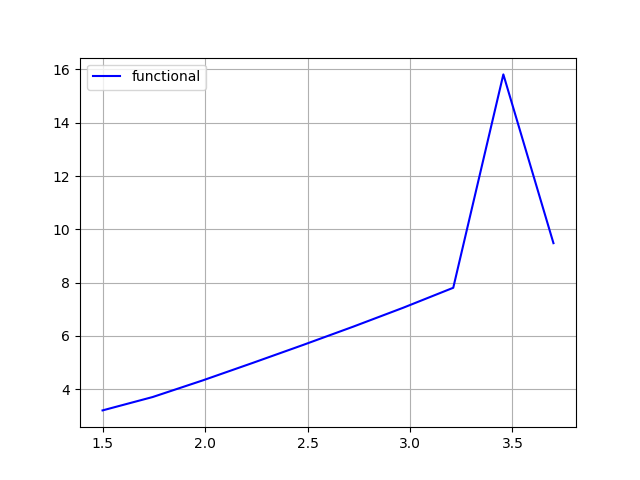
\includegraphics[scale=0.5]{fig/functional_1_5-3_7_50.png}
\caption{}
\end{figure}
\end{frame}

\begin{frame}{Примеры численного решения для поворотов на малые углы - первый случай, когда $\alpha_3$ фиксирована}
\begin{figure}[H]
\center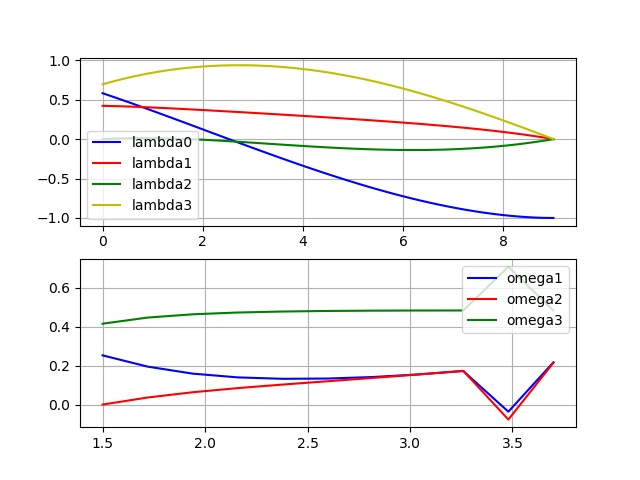
\includegraphics[scale=0.5]{fig/ivp_and_control_1_5-3_7_50.png}
\caption{}
\end{figure}
\end{frame}

\begin{frame}{Примеры численного решения для поворотов на малые углы - второй случай, когда $\alpha_2$ фиксирована}
\begin{figure}[H]
\center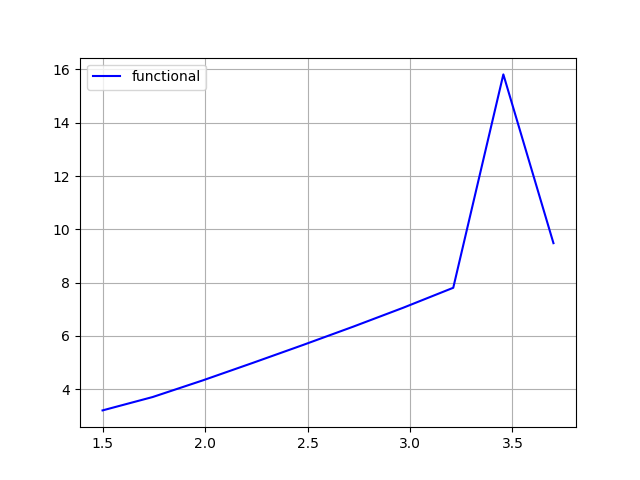
\includegraphics[scale=0.5]{fig/functional_1_5-3_7_50.png}
\caption{}
\end{figure}
\end{frame}

\begin{frame}{Примеры численного решения для поворотов на малые углы - второй случай, когда $\alpha_2$ фиксирована}
\begin{figure}[H]
\center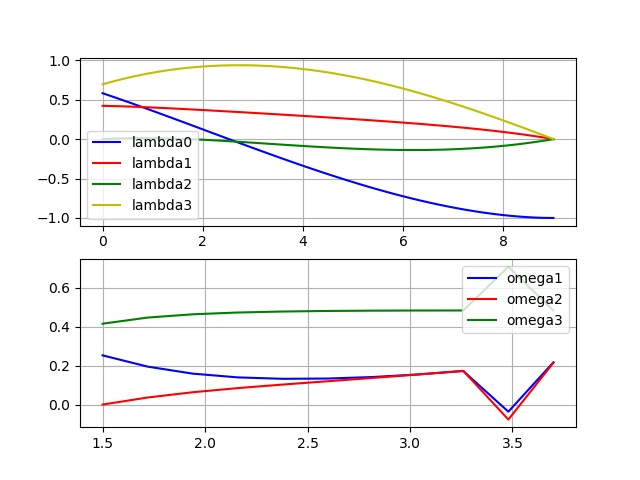
\includegraphics[scale=0.5]{fig/ivp_and_control_1_5-3_7_50.png}
\caption{}
\end{figure}
\end{frame}

\begin{frame}
\frametitle{Примеры численного решения для поворотов на большие углы - третий случай, когда $\alpha_3$ фиксирована}
\begin{figure}[H]
\center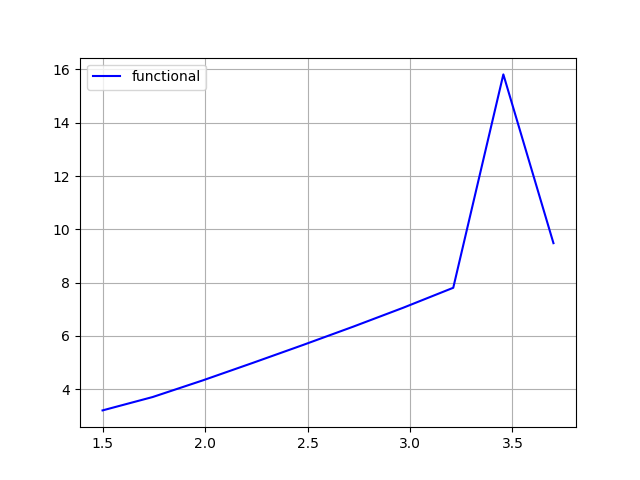
\includegraphics[scale=0.5]{fig/functional_1_5-3_7_50.png}
\caption{}
\end{figure}
\end{frame}

\begin{frame}{Примеры численного решения для поворотов на большие углы - третий случай, когда $\alpha_3$ фиксирована}
\begin{figure}[H]
\center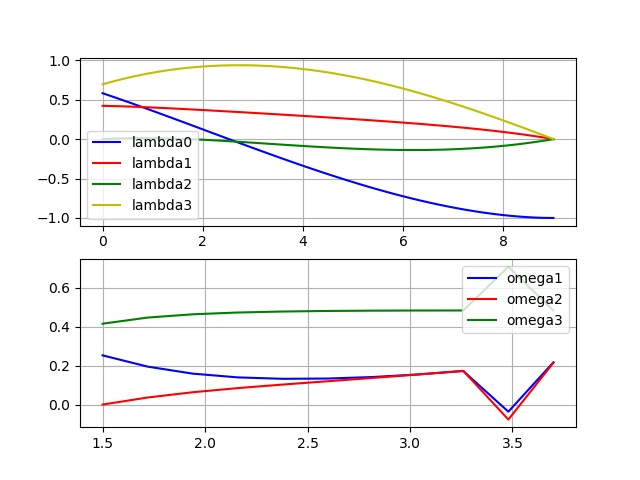
\includegraphics[scale=0.5]{fig/ivp_and_control_1_5-3_7_50.png}
\caption{}
\end{figure}
\end{frame}

\begin{frame}{Примеры численного решения для поворотов на большие углы - четвертый случай, когда $\alpha_2$ фиксирована}
\begin{figure}[H]
\center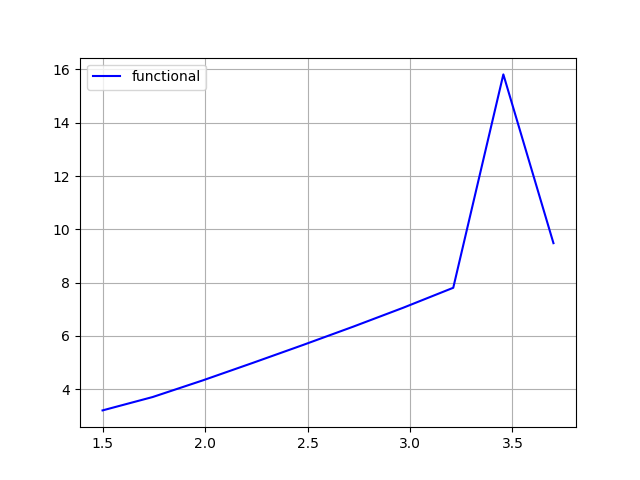
\includegraphics[scale=0.5]{fig/functional_1_5-3_7_50.png}
\caption{}
\end{figure}
\end{frame}

\begin{frame}{Примеры численного решения для поворотов на большие углы - четвертый случай, когда $\alpha_2$ фиксирована}
\begin{figure}[H]
\center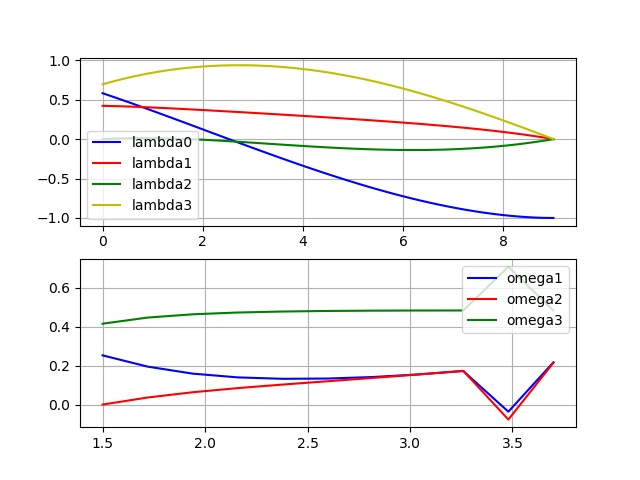
\includegraphics[scale=0.5]{fig/ivp_and_control_1_5-3_7_50.png}
\caption{}
\end{figure}
\end{frame}

\begin{frame}{База данных для хранения графиков}
\end{frame}

\begin{frame}[standout]
Спасибо за внимание!
\end{frame}

\end{document}
